\hypertarget{jggsal_8h}{}\section{Referencia del Archivo include/jggsal.h}
\label{jggsal_8h}\index{include/jggsal.\+h@{include/jggsal.\+h}}


Software Abstraction Layer.  


Gráfico de los archivos que directa o indirectamente incluyen a este archivo\+:\nopagebreak
\begin{figure}[H]
\begin{center}
\leavevmode
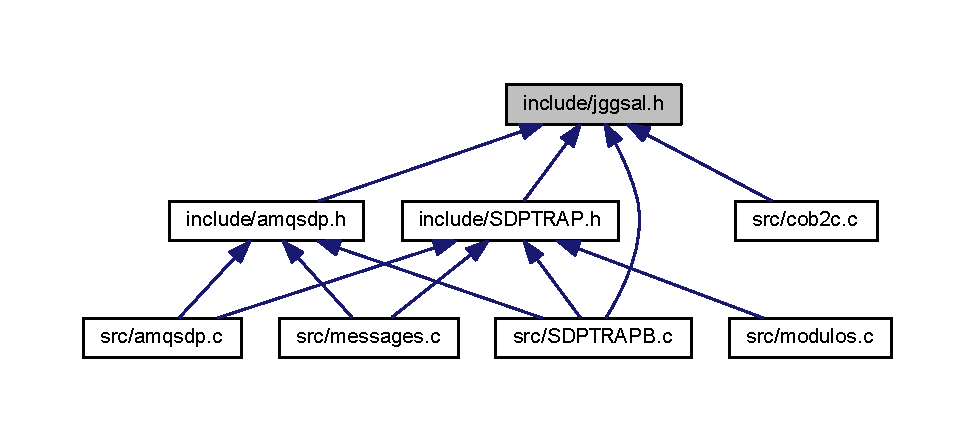
\includegraphics[width=350pt]{jggsal_8h__dep__incl}
\end{center}
\end{figure}


\subsection{Descripción detallada}
Software Abstraction Layer. 

Componente de compatibilidad entre sistemas operativos Redefine las funciones del runtime en funcion del Sistema Operativo Cuando es necesario, jggsal.\+c actua como wrapper de la funcion objetivo.

De esta manera se eliminan los bloques \#ifdef {\itshape O\+S} del codigo fuente

O\+J\+O\+: N\+O P\+U\+E\+D\+E L\+L\+A\+M\+A\+R\+S\+E S\+A\+L P\+O\+R\+Q\+U\+E L\+O U\+T\+I\+L\+I\+Z\+A W\+I\+N\+D\+O\+W\+S

\begin{DoxyAuthor}{Autor}
\+: Javier Gonzalez 
\end{DoxyAuthor}
\begin{DoxyDate}{Fecha}
\+: 01/03/15 
\end{DoxyDate}
\begin{DoxyVersion}{Versión}
\+: 1.\+0 
\end{DoxyVersion}
